% Copyright (c) 2021 ArSysOp
%
% This program and the accompanying materials are made available under the
% terms of the Eclipse Public License 2.0 which is available at
% https://www.eclipse.org/legal/epl-2.0/.
%
% SPDX-License-Identifier: EPL-2.0

\documentclass[12pt]{report}

\usepackage{color}
\usepackage[usenames,dvipsnames,svgnames,table]{xcolor}

\usepackage{graphicx}
\graphicspath{{../../i/common/}}

\usepackage{hyperref}
\hypersetup{colorlinks=true,
linkcolor=black,
urlcolor=gray}

\usepackage{fancyhdr}
\pagestyle{fancy}
\fancyhf{}
\lhead{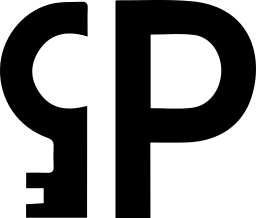
\includegraphics[width=13pt]{glyph}}
\rhead{\leftmark}
\lfoot{\thepage}
\rfoot{Eclipse Passage}
\renewcommand{\chaptermark}[1]{\markboth{#1}{}}
\renewcommand{\headrulewidth}{0.5pt}
\renewcommand{\footrulewidth}{0.5pt}

\fancypagestyle{plain}{
    \fancyhf{}
    \lhead{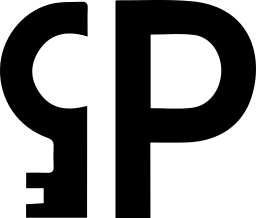
\includegraphics[width=13pt]{glyph}}
    \rhead{\leftmark}
    \lfoot{\thepage}
    \rfoot{Eclipse Passage}
    \renewcommand{\headrulewidth}{0.5pt}
    \renewcommand{\footrulewidth}{0.5pt}
}

\setlength{\headheight}{16pt}

\title{Eclipse Passage Floating License Server}
\author{ArSysOp}
\date{07 Jule 2021}

\begin{document}

\begin{titlepage}
    \begin{center}
        \vspace*{1cm}

        \Huge \textbf{Eclipse Passage}
        
        \Huge \textbf{Floating License Server}
        
        \Huge \textbf{Administration Guide}

        \vspace{0.5cm}

        \Large \today

        \vfill

        
\includegraphics[width=5cm]{passage}

        \vfill

        \Large ArSysOp
    \end{center}
\end{titlepage}

\tableofcontents
\markboth{Table of Contents}{}

\addcontentsline{toc}{chapter}{Overview}
\chapter*{Overview}
Eclipse Passage is a set of tools and libraries providing rich and easily adaptable capabilities 
to declare and control licensing constraints.

\addcontentsline{toc}{section}{Contribution}
\section*{Contribution}
If you found a mistake in the text or just want to improve this user guide, feel free to contribute on \href{https://github.com/eclipse-passage/passage-docs}{Github} repository.

Also we want to remind that Eclipse Passage is an open-source project, so you can always contribute to the project \href{https://github.com/eclipse-passage/passage}{itself}.

\addcontentsline{toc}{section}{License}
\section*{License}
These materials are made available under the terms of the \href{https://www.eclipse.org/legal/epl-2.0/}{Eclipse Public License 2.0}.

\addcontentsline{toc}{chapter}{How floating licensing works}
\chapter*{How floating licensing works}

As opposed to personal licensing, where a user of a product-under-licensing 
gets their own license and hosts it close to the product for single use,
floating licensing delegates actual license packs hosting and executing to a dedicated agent - \textbf{Floating License Server}. 

This allows number of users to exploit their installations of the product simultaneously in the scope of a single floating license pack. 

\addcontentsline{toc}{section}{Floating License Server}
\section*{Floating License Server}

The Server, that is installed somewhere in the reach, 
\begin{itemize}
    \item hosts all floating license packs and
    \item responds to \textit{give me permission to use this feature} requests from the product's users via http.
\end{itemize}

\addcontentsline{toc}{section}{Communication with the Server}
\section*{Communication with the Server}

The product 
\begin{itemize}
    \item asks the Server for a grant on a particular feature and, 
    \item if succeed, proceeds with the feature and then, 
    \item when it's over, releases the grant.
\end{itemize} 

The Server can lease several grants for the same feature at the same time, as hosted floating licence packs permit.

\addcontentsline{toc}{section}{Full floating licensing workflow}
\section*{Full floating licensing workflow}

There are four \textit{actors} in the floating licensing workflow:

\begin{itemize}

	\item \textit{product development and management}, where
		\begin{itemize}
		    \item management \textit{defines products}, \textit{feature sets} and \textit{product release plan} and
		    \item development
		    	\begin{itemize}
		      		\item \textit{declares licensing requirements} in the product codebase,
		      		\item  \textit{covers feature usages with licensing protection},
		      		\item  \textit{configures the product to use Floating License Server};
		      	\end{itemize}
      	\end{itemize}
	\item \textit{operator}, who~\hyperref[ch:issue-flp]{issues} a~\hyperref[ch:flp]{floating license pack} and delivers it,  
	\item \textit{agent}, who~\hyperref[ch:install-fls]{installs} and~\hyperref[ch:run-fls]{runs} a Floating License Server,
	\item \textit{client} as a representative of set of the product \textit{users}, who 
    deploys personal part of a \textit{floating license pack}.

\end{itemize} 

\addcontentsline{toc}{chapter}{Floating license pack}
\chapter*{Floating license pack} \label{ch:flp}

\addcontentsline{toc}{chapter}{Issue floating license pack}
\chapter*{Issue Floating license pack} \label{ch:issue-flp}

\addcontentsline{toc}{chapter}{Install Floating License Server}
\chapter*{Install Floating License Server} \label{ch:install-fls}

\addcontentsline{toc}{chapter}{Run Floating License Server}
\chapter*{Run Floating License Server} \label{ch:run-fls}

\end{document}
